The goal of attackers who attempt to corrupt the memory of a process is usually to take control of it such that they can run with the privileges of the process and execute attacker-specified code. These attacks are made possible by mixing data and control in memory and allowing users to overwrite control data.

Therefore, we need to look at the defenses against such attacks.

\section{Defenses}
We want to make sure that for memory accesses, including read, write, and execute, there is no access to `undefined' memory. Note that `undefined' is with respect to the semantics of the programming language. To make sure the code executes safely, we utilize a module-by-module analysis.

\subsection{Conditions}
Here we discuss two conditions: preconditions and postconditions.

\textbf{Preconditions} describe what must hold for a function or statement to operate correctly. Formally, a precondition is an assertion that must hold about the inputs of a function for it to work correctly. The caller must satisfy the precondition, and the callee may assume that the precondition is met.

\textbf{Postconditions} describe what holds after the function returns or the statement is executed. A postcondition is an assertion that must hold after a function returns. The caller may assume that the postcondition holds, while the callee must ensure that the postcondition holds. For consecutive statements, the postcondition of statement 1 should logically imply the precondition of statement 2.

There are also \textbf{invariants}, which are conditions that always hold at a given point in a function.

For example, consider

\begin{verbatim}
int deref(int *p) {
  return *p;
}
\end{verbatim}

The precondition that must hold is that the pointer \texttt{p} is not \texttt{NULL} and is valid. For

\begin{verbatim}
void *my_malloc(size_t n) {
  void *p = malloc(n);
  if (!p) { 
    perror("malloc"); 
    exit(1); 
  }
  return p;
}
\end{verbatim}

The postcondition here is that the return value is not \texttt{NULL} and \texttt{p} is a valid pointer.

In general, the correctness proof strategy for memory safety is to identify each memory access point, write down the precondition it requires, and propagate the requirement up to the beginning of the function.

In cases with more complicated loops, induction might be used. The base case corresponds to the first entrance into the loop, and the induction step shows that the postcondition of the last statement in the loop, together with the loop test condition, implies the invariant.

\subsection{Approaches}

To defend against attacks due to memory corruption, we have two approaches.

\textbf{Prevention}

We aim to write bug-free programs, or rewrite programs in a memory-safe language that automatically checks boundaries and does not allow unsafe pointer arithmetic. We can also analyze programs for potential vulnerabilities before execution, prevent attack code execution, and make exploitation harder.

\textbf{Detection}

We detect attacks by performing security checks during program execution, such as detecting abnormal sequences of executed instructions and checking for integrity violations.

We now look at four types of defense.

\subsection{Canary}
\begin{minipage}{0.4\textwidth}
Canaries are placed in stack frames to prevent and detect overwriting of the return address on the stack. StackGuard inserts a canary before the return address in each stack frame, such that when the function returns, the canary value is verified against the stored value. This acts as a runtime check for stack integrity.\\[3pt]
There are different types of canaries:\\[3pt]
1. \textbf{Terminator Canary}\\[3pt]
This type of canary uses \texttt{NULL} (\texttt{0x00}), \texttt{CR} (\texttt{0x0d}), \texttt{LF} (\texttt{0x0a}), and \texttt{EOF} (\texttt{0xff}). String functions will not copy beyond a terminator, so attackers cannot use such functions to overwrite the return address.
\end{minipage}
\begin{minipage}{0.6\textwidth}
\begin{figure}[H]
  \centering
  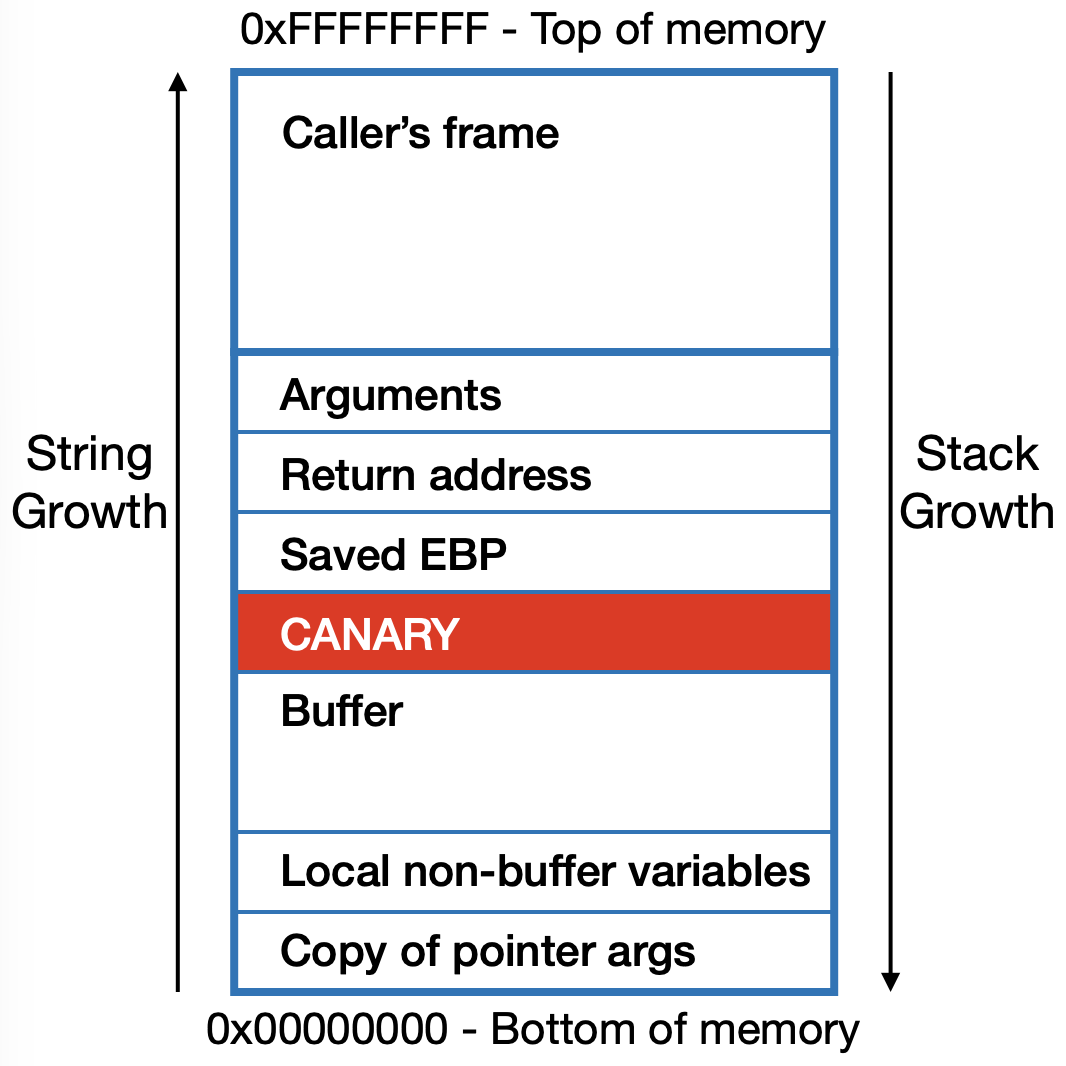
\includegraphics[width=0.6\textwidth]{Figure/ProtectionCanary.png}
  \caption{Stack with canary}
\end{figure}
\end{minipage}

However, terminator canaries are not completely random. For example, there are always fixed zero bytes, making it easier to guess the canary and potentially brute-force it.

2. \textbf{Random Canary}

A random value is chosen at program startup and stored in a location known only to the validation code, often protected using unmapped pages.

3. \textbf{XOR Canary}

This uses \texttt{random value \(\oplus\) return address}.

There are also limitations to canaries. Canaries do not provide full protection because they can be learned. For example, there might be format string vulnerabilities or information leakage, and canaries can also be overwritten. Moreover, other pointers can still be overwritten. For example, a function pointer in the stack frame can be overwritten.

Canaries can also be bypassed by overflowing a pointer used as the destination of a \texttt{strcpy()}-like function. Some stack-smashing techniques can overwrite the return address without touching the canary (note that the XOR canary was introduced to protect against this attack). Also, enabling canary protection requires recompiling the program, which can be expensive.

\subsection{Non-Executable Memory}

In order to prevent attacker-supplied code from executing, the operating system can mark the stack and heap as non-executable.

\begin{remark}
  Linux leverages the NX (No-eXecute) bit in the page table entry to mark certain memory areas as non-executable. Windows implements this mechanism using Data Execution Prevention (DEP), which can emulate the mechanism if the NX bit is not supported by the processor. OpenBSD implements W \(\oplus\) X, which enforces that a page is either writable or executable, but not both.
\end{remark}

These mechanisms aim to ensure that no memory region is both writable and executable. However, some applications may require writable memory that is also executable. In addition, attackers can still hijack the control flow of a vulnerable application even if the memory is non-executable, for example, via return-to-libc or return-oriented programming (ROP).

If the memory is non-executable, attackers cannot launch code-injection attacks. However, they can still hijack the control flow by using existing functions or code snippets in libraries and chaining them together to perform the desired tasks.

\subsection{Address Space Layout Randomization (ASLR)}

This defense maps the stack, heap, code, and shared libraries to random locations in the process memory. The library code needs to be position-independent; otherwise, runtime mapping may incur overhead. This makes jumping to a library function more difficult.

In Linux, ASLR is enabled by default. It is implemented by the kernel in collaboration with the ELF loader.

To exploit ASLR, brute-forcing can be used if the entropy is low, i.e.\ if it is possible to limit the variation space.

\begin{remark}
  In security, entropy refers to how many possible values something can take. High entropy means many possibilities, making it hard to guess. Low entropy means fewer possibilities, making it easier to guess via brute-force.
\end{remark}

\subsection{Control Flow Integrity}

Previously, we discussed the control flow graph (CFG). Programs have a CFG, and control-hijacking attacks usually result in execution paths that do not exist in the CFG. Therefore, control flow integrity (CFI) ensures that the application follows only the control flows specified by the CFG.

To enforce CFI, the CFG is built at compile time, and the application is instrumented to check at runtime the validity of each control transfer.

For example, in Windows 10, Control Flow Guard (CFG) prevents jumping to invalid locations through indirect calls by checking against a bitmap of all valid function entry points in the executable. However, it does not prevent an attacker from jumping to a valid but unintended function, so it is difficult to statically build a fully accurate CFG.